\section{First night train trip down Captain Kangaroo}

\subsection{13--14/08/09}

\margininbox{Kill'em All}{
     \begin{itemize}
    \item Tharatorn Supasiti
    \item Tim Osborne
    \end{itemize}}{\explo}

Tim and I descended down \passage{Captain Kangaroo} for the second and the
last time in this expo. Our two main objectives were to dislodge a
boulder at the pitch head of \passage{Kill'em All} and to further push the
bottom of \passage{Happy Monday} as left by Jana and Dan previously. For
the latter objective, we expected a connection with the main \passage{Gardeners' World} system
as explored in early 00's from the most recent cave data.

Somehow we ended up on a night train, which is my first. We took off
from the bivvi after sunset. While changing into our respective caving
gears at \passage{Gardeners' World} entrance, we knew that those left at the bivvi were having
fun with newly-acquired laser by a green beam that pierced through
the mountain's night fog.

\begin{marginfigure}
\checkoddpage \ifoddpage \forcerectofloat \else \forceversofloat \fi
\centering
 \frame{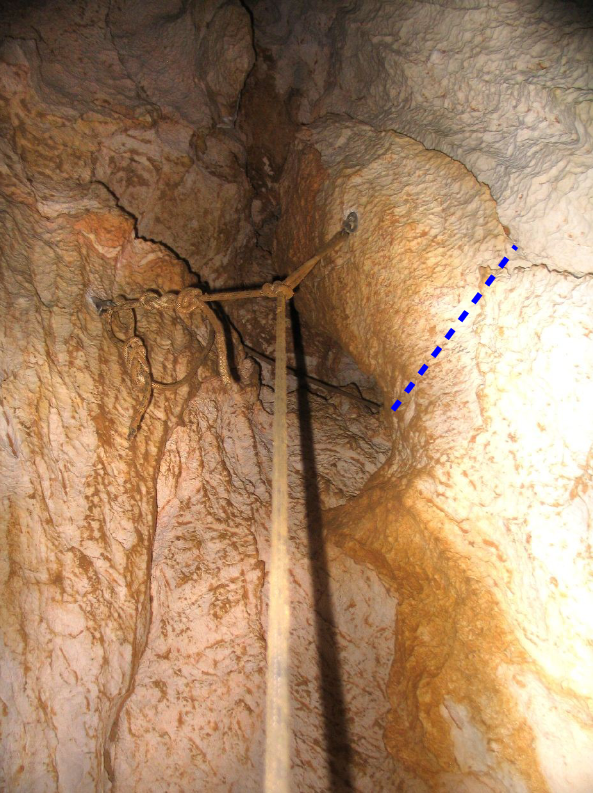
\includegraphics[width=\linewidth]{2009/night_train/Screenshot 2023-10-30 at 12-30-29 Slide 1 - BCRA 2009 - Jarvist Frost.pdf.png}} 
 \caption{The \protect\passage{Kill'em All} pitch head from below with the rock of concern highlighted by the blue line. \pic{Jarvist Frost}}
 \label{kill'em all crack}
\end{marginfigure}

Upon arriving \passage{Metal Camp}, we headed straight to complete the
first objective. I crawled through a tight pitch head and at once I knew
that I have arrived at \passage{Kill'em All} by the Y-hang that was set
below the ledge. A haunted memory of my previous struggles to pass
through this head in either ways, came flooding back. I could only take
comfort in knowing that today would be the last time that anyone will
ever have to experience this struggle between rock (and gravity) and man.

On the surface, during the previous days, there was a growing concern by
numerous parties that had to pass through this head that the rock on
which one of the two bolts that made up the Y-hang has developed a
widening crack. It was only a matter of time until this boulder would
dislodge unto unfortunate souls still half-way through the
descent/ascent. So, it was Tim and I's job to secure this passage.

Since I am small to allow myself to swing a hammer at the head, I was
assigned with the chiselling duty. After derigging the pitch, it didn't
take too long with chisel in one hand and a lump hammer in the other to
dislodge a table size boulder down the pitch. And it crashed with a loud
thud that echoed through the chamber below.

Half an hour later, after Tim put a new bolt, we returned to the camp
considering a job well-done.

\name{Tharatorn Supasiti}


\subsection{14--15/08/09}

\margininbox{Hanging Garden}{
     \begin{itemize}
    \item Tim Osborne
    \item Tharatorn Supasiti
    \end{itemize}}{\explo}

The next night (or day by our standard), we continued Dan and Jana's
lead down \passage{Happy Monday} through a gap between loose rock and its
wall. Little did we know that we, indeed, were kept up there by pure
friction on the cavern wall. A double hammer action quickly led us into
a chamber below \passage{Happy Monday}. I was the first to descend into the
unknown chamber.

Upon looking towards the ceiling, I noticed three large boulders
suspended mid-air that formed the roof of this chamber. And the only
thing that prevent the roof from collapsing is the friction between
boulders and the cavern wall. The name for this chamber is obviously
``\passage{Hanging Garden}'' and I knew that I had to get out of here ASAP.

\margininbox{Free Amalgamation}{
     \begin{itemize}
    \item Tim Osborne
    \item Tharatorn Supasiti
    \end{itemize}}{\explo}

The way onward was obvious. We followed the rift to a 5 m pitch that
dropped into a flat white floor, where water flew through. A bit further
down, having found a spitz on a wall, \bignote{we realised that we had made a
CONNECTION!} (It wasn't until the next trip that the survey was tied in.
We couldn't find a survey station.)

I went back up the same rift, while Tim attempted to rig a line across
to a window opposite the rift we were in. After shivering in the cold
for hours (it was 4am), my morale was at the lowest. And I begged Tim to
survey and get out.

During surveying the new section, a loose fell from the pitch head and
sliced through our tape. Luckily, that was near the end of our survey.

The journey back to the camp was arguably one of my most hallucinating
experience I ever I encountered in the cave. Having been broken at 4am,
my body refused to answer the call of duty to migrate towards bed. I
didn't remember how I got back to the camp, but got back we did.
Exhausted, I resorted to ignore food and went straight to sleep, while
Tim sorted out his bowel less than ten metres away\ldots{}

\tweet{4:04PM Aug 15, 2009}{Latest camp finds HANGING GARDEN, a way through the boulder choke at the bottom of HM to find bolts on FALLS ROAD off F-SHIP gallery.}

We exited the cave by 4am.

After 55 hours of holding it in, the shit pit finally called me\ldots{}

NB: I thought to myself then, never will I go on a night train again.
This was broken in 2012. I only went on night train trips.

\name{Tharatorn Supasiti}


\begin{figure*}
\checkoddpage \ifoddpage \forcerectofloat \else \forceversofloat \fi
\centering
\begin{subfigure}[t]{0.49\textwidth}
    \centering
        \frame{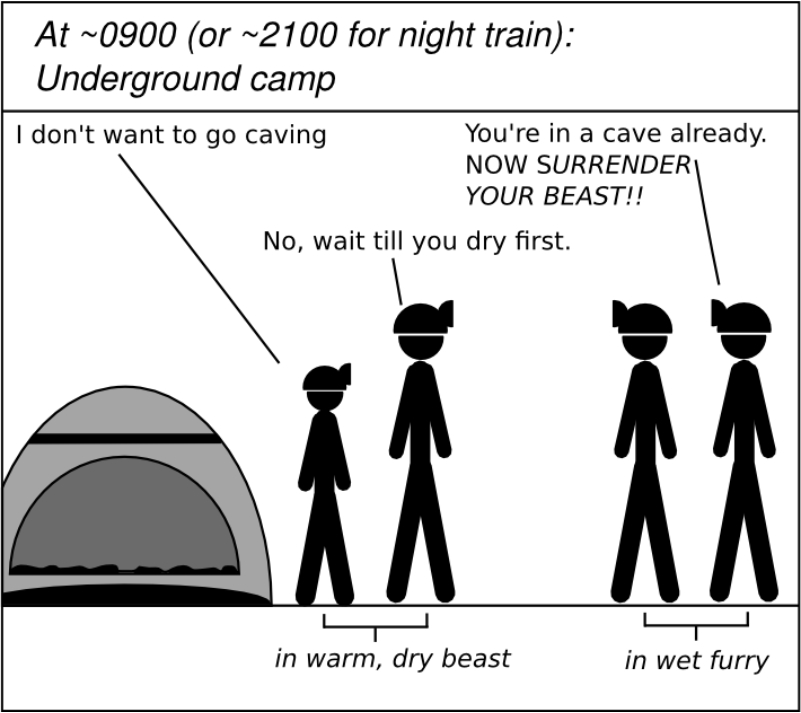
\includegraphics[width=\linewidth]{2009/night_train/Screenshot 2023-10-29 at 12-37-50 Slide 1 - BCRA 2009 - Jarvist Frost.pdf.jpg}} 
        \caption{} \label{beast swap 1}
    \end{subfigure}
    \hfill
    \begin{subfigure}[t]{0.49\textwidth}
    \centering
        \frame{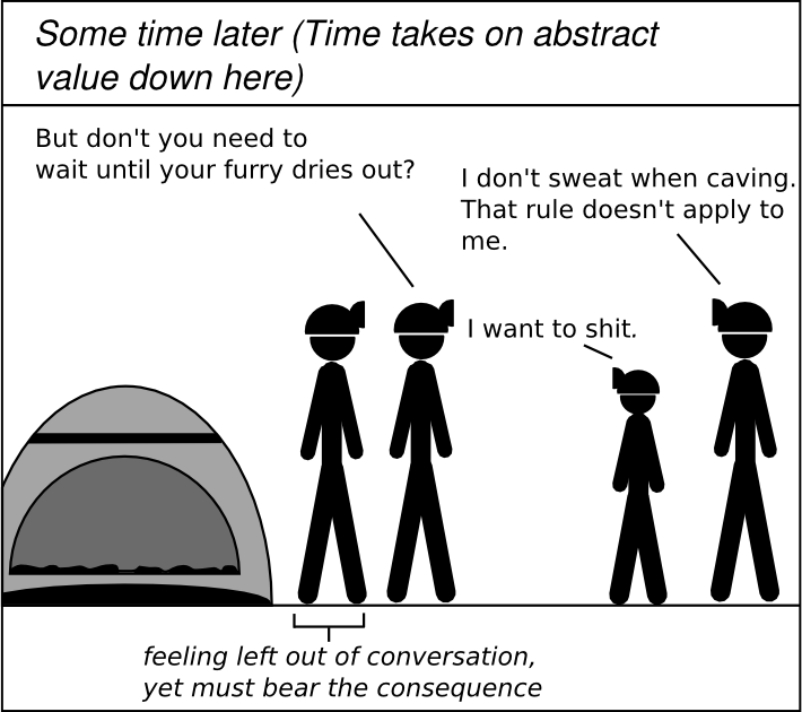
\includegraphics[width=\linewidth]{2009/night_train/Screenshot 2023-10-29 at 12-38-08 Slide 1 - BCRA 2009 - Jarvist Frost.pdf.jpg}} 
        \caption{} \label{beast swap 2}
    \end{subfigure}
    \caption{The BEAST exchange protocol in \passage{Metal Camp}. \textit{(a)} Team A doesn't want to go caving. Team B wants the beastly comf. \textit{(b)} The opposite of \textit{(a)}. \pen{Tharatorn Supasiti}}
    \label{beast cartoon}
\end{figure*}


%\subsection{logbook - 13--14/08/09 - Thara and Tim}

%Fixed \passage{Kill 'em All} - dislodged a large boulder down the pitch. New
%bolt was put in place.

%14-15: Thara and Tim Continued down Dan's lead down one more pitch --
%double hammer action lead into a chamber clearly below \passage{Happy
%Monday}. Hanging death a size of whole chamber kept everything from
%falling down. It's like anti-gravity room where rock just floats itself
%in the sky. Followed an obvious rift to a 5 m pitch into another
%chamber. Flat floor with a lot water coming through just like Yorkshire
%caves. Walked further downstream and found spitz -- clear someone has
%been here before. Back to chamber - Tim tried to rig a traverse line
%across to another lead half finished before heading off.

%Thara was completely broken by the top of \passage{Happy Monday} while
%Tim's bowel rumbled once again. Great find and survey.

%Left: rope some bolting kit + tape + sling at the bottom of \passage{happy
%monday}. Hammer and chisel at the top of \passage{Kill'em All}

%PS: From final pitch, there is a traverse line to the right. It is not
%great as a proper traverse, but if you descend the main pitch, you can
%use the traverse line with a cows tail to reach the other side. There is
%a bolt to go down from there but it needs a backup. Once rigged it would
%be better to descend main rope then up the other one.